%%%%%%%%%%%%%%%%%%%%%%%%%%%%%%%%%%%%%%%%%
% Masters/Doctoral Thesis 
% LaTeX Template
% Version 2.2 (21/11/15)
%
% This template has been downloaded from:
% http://www.LaTeXTemplates.com
%
% Version 2.x major modifications by:
% Vel (vel@latextemplates.com)
%
% This template is based on a template by:
% Steve Gunn (http://users.ecs.soton.ac.uk/srg/softwaretools/document/templates/)
% Sunil Patel (http://www.sunilpatel.co.uk/thesis-template/)
%
% Template license:
% CC BY-NC-SA 3.0 (http://creativecommons.org/licenses/by-nc-sa/3.0/)
%
%%%%%%%%%%%%%%%%%%%%%%%%%%%%%%%%%%%%%%%%%

%----------------------------------------------------------------------------------------
%	PACKAGES AND OTHER DOCUMENT CONFIGURATIONS
%----------------------------------------------------------------------------------------

\documentclass[
11pt, % The default document font size, options: 10pt, 11pt, 12pt
%oneside, % Two side (alternating margins) for binding by default, uncomment to switch to one side
english, % ngerman for German
singlespacing, % Single line spacing, alternatives: onehalfspacing or doublespacing
%draft, % Uncomment to enable draft mode (no pictures, no links, overfull hboxes indicated)
%nolistspacing, % If the document is onehalfspacing or doublespacing, uncomment this to set spacing in lists to single
%liststotoc, % Uncomment to add the list of figures/tables/etc to the table of contents
%toctotoc, % Uncomment to add the main table of contents to the table of contents
%parskip, % Uncomment to add space between paragraphs
%nohyperref, % Uncomment to not load the hyperref package
headsepline, % Uncomment to get a line under the header
]{MastersDoctoralThesis} % The class file specifying the document structure

\usepackage[utf8]{inputenc} % Required for inputting international characters
\usepackage[T1]{fontenc} % Output font encoding for international characters

\usepackage{palatino} % Use the Palatino font by default

\usepackage[backend=bibtex,bibstyle=ieee, citestyle=numeric-comp,natbib=true]{biblatex} % User the bibtex backend with the authoryear citation style (which resembles APA)

\addbibresource{example.bib} % The filename of the bibliography

%----------------------------------------------------------------------------------------
%	MARGIN SETTINGS
%----------------------------------------------------------------------------------------

\geometry{
	paper=a4paper, % Change to letterpaper for US letter
	inner=2.5cm, % Inner margin
	outer=3.8cm, % Outer margin
	bindingoffset=2cm, % Binding offset
	top=1.5cm, % Top margin
	bottom=1.5cm, % Bottom margin
	%showframe,% show how the type block is set on the page
}

%----------------------------------------------------------------------------------------
%	THESIS INFORMATION
%----------------------------------------------------------------------------------------

\thesistitle{Machine learning techniques for flow-based network intrusion detection systems} % Your thesis title, this is used in the title and abstract, print it elsewhere with \ttitle
\supervisor{Prof. Dr. Peter \textsc{Quax} \\ Prof. Dr. Wim \textsc{Lamotte} \\ Bram \textsc{Bonne} \\ Pieter \textsc{Robyns}} % Your supervisor's name, this is used in the title page, print it elsewhere with \supname
\examiner{} % Your examiner's name, this is not currently used anywhere in the template, print it elsewhere with \examname
\degree{Bachelor of Science in Computer Science} % Your degree name, this is used in the title page and abstract, print it elsewhere with \degreename
\author{Axel \textsc{Faes}} % Your name, this is used in the title page and abstract, print it elsewhere with \authorname
\addresses{} % Your address, this is not currently used anywhere in the template, print it elsewhere with \addressname

\subject{Computer Science} % Your subject area, this is not currently used anywhere in the template, print it elsewhere with \subjectname
\keywords{} % Keywords for your thesis, this is not currently used anywhere in the template, print it elsewhere with \keywordnames
\university{\href{http://www.uhasselt.be}{University of Hasselt}} % Your university's name and URL, this is used in the title page and abstract, print it elsewhere with \univname
\department{{Computer Science}} % Your department's name and URL, this is used in the title page and abstract, print it elsewhere with \deptname
\faculty{{Wetenschappen}} % Your faculty's name and URL, this is used in the title page and abstract, print it elsewhere with \facname

\hypersetup{pdftitle=\ttitle} % Set the PDF's title to your title
\hypersetup{pdfauthor=\authorname} % Set the PDF's author to your name
\hypersetup{pdfkeywords=\keywordnames} % Set the PDF's keywords to your keywords

\renewcommand{\cleardoublepage}{\clearpage}

\begin{document}

\frontmatter % Use roman page numbering style (i, ii, iii, iv...) for the pre-content pages

\pagestyle{plain} % Default to the plain heading style until the thesis style is called for the body content

%----------------------------------------------------------------------------------------
%	TITLE PAGE
%----------------------------------------------------------------------------------------

\begin{titlepage}
\begin{center}

\textsc{\LARGE \univname}\\[1.5cm] % University name

\textsc{\Large Bachelor Thesis}\\[0.5cm] % Thesis type

\HRule \\[0.4cm] % Horizontal line
{\huge \bfseries \ttitle}\\[0.4cm] % Thesis title
\HRule \\[1.5cm] % Horizontal line
 
\begin{minipage}{0.4\textwidth}
\begin{flushleft} \large
\emph{Author:}\\
{\authorname} % Author name - remove the \href bracket to remove the link
\end{flushleft}
\end{minipage}
\begin{minipage}{0.4\textwidth}
\begin{flushright} \large
\emph{Supervisor:} \\
{\supname} % Supervisor name - remove the \href bracket to remove the link  
\end{flushright}
\end{minipage}\\[2.5cm]
 
\large \textit{Bachelorproef voorgedragen tot het behalen van de graad van bachelor in de informatica/ICT/kennistechnologie}\\[0.3cm]
\large \textit{A thesis submitted in fulfillment of the requirements\\ for the degree of \degreename}\\[0.3cm] % University requirement text
%\textit{in the}\\[0.4cm]
%\groupname\\\deptname\\[2cm] % Research group name and department name
 ~\\[1cm]
 
{\large \today}\\[2cm] % Date
%\includegraphics{Logo} % University/department logo - uncomment to place it
 
\includegraphics[width=0.7\textwidth]{LOGO}~\\[1cm]

\vfill
\end{center}
\end{titlepage}

%----------------------------------------------------------------------------------------
%	DECLARATION PAGE
%----------------------------------------------------------------------------------------

\begin{declaration}
\addchaptertocentry{\authorshipname}

\noindent I, \authorname, declare that this thesis titled, \enquote{\ttitle} and the work presented in it are my own. I confirm that:

\begin{itemize} 
\item This work was done wholly or mainly while in candidature for a bachelor degree at this University.
\item Where any part of this thesis has previously been submitted for a degree or any other qualification at this University or any other institution, this has been clearly stated.
\item Where I have consulted the published work of others, this is always clearly attributed.
\item Where I have quoted from the work of others, the source is always given. With the exception of such quotations, this thesis is entirely my own work.
\item I have acknowledged all main sources of help.
\item Where the thesis is based on work done by myself jointly with others, I have made clear exactly what was done by others and what I have contributed myself.\\
\end{itemize}
 
\noindent Signed:\\
\rule[0.5em]{25em}{0.5pt} % This prints a line for the signature
 
\noindent Date:\\
\rule[0.5em]{25em}{0.5pt} % This prints a line to write the date
\end{declaration}

%\cleardoublepage

%%----------------------------------------------------------------------------------------
%%	QUOTATION PAGE
%%----------------------------------------------------------------------------------------
%
%\vspace*{0.2\textheight}
%
%\noindent\enquote{\itshape Thanks to my solid academic training, today I can write hundreds of words on virtually any topic without possessing a shred of information, which is how I got a good job in journalism.}\bigbreak
%
%\hfill Dave Barry

%----------------------------------------------------------------------------------------
%	ABSTRACT PAGE
%----------------------------------------------------------------------------------------

\begin{abstract}
\addchaptertocentry{\abstractname} % Add the abstract to the table of contents



\end{abstract}

%----------------------------------------------------------------------------------------
%	ACKNOWLEDGEMENTS
%----------------------------------------------------------------------------------------

\begin{acknowledgements}
\addchaptertocentry{\acknowledgementname} % Add the acknowledgements to the table of contents

%The acknowledgments and the people to thank go here, don't forget to include your project advisor\ldots

\end{acknowledgements}

%----------------------------------------------------------------------------------------
%	LIST OF CONTENTS/FIGURES/TABLES PAGES
%----------------------------------------------------------------------------------------

\tableofcontents % Prints the main table of contents

\listoffigures % Prints the list of figures

\listoftables % Prints the list of tables

%----------------------------------------------------------------------------------------
%	ABBREVIATIONS
%----------------------------------------------------------------------------------------

\begin{abbreviations}{ll} % Include a list of abbreviations (a table of two columns)

\textbf{IDS} & \textbf{I}ntrusion \textbf{D}etection \textbf{S}ystem\\
\textbf{IPS} & \textbf{I}ntrusion \textbf{P}revention \textbf{S}ystem\\
\textbf{IDPS} & \textbf{I}ntrusion \textbf{D}etection (and) \textbf{P}revention \textbf{S}ystem\\
\textbf{NIDS} & \textbf{N}etwork (based) \textbf{I}ntrusion \textbf{D}etection \textbf{S}ystem\\
\textbf{HIDS} & \textbf{H}ost (based) \textbf{I}ntrusion \textbf{D}etection \textbf{S}ystem\\
\\
\textbf{DDOS} & \textbf{D}tributed \textbf{D}enial \textbf{o}f \textbf{S}ervice
\\
\textbf{ML} & \textbf{M}achine \textbf{L}earning\\
%\textbf{WSF} & \textbf{W}hat (it) \textbf{S}tands \textbf{F}or\\

\end{abbreviations}

%----------------------------------------------------------------------------------------
%	SYMBOLS
%----------------------------------------------------------------------------------------

\begin{symbols}{lll} % Include a list of Symbols (a three column table)

%$a$ & distance & \si{\meter} \\
%$P$ & power & \si{\watt} (\si{\joule\per\second}) \\
%Symbol & Name & Unit \\

\addlinespace % Gap to separate the Roman symbols from the Greek

%$\omega$ & angular frequency & \si{\radian} \\

\end{symbols}

%----------------------------------------------------------------------------------------
%	DEDICATION
%----------------------------------------------------------------------------------------

%\dedicatory{For/Dedicated to/To my\ldots} 

%----------------------------------------------------------------------------------------
%	THESIS CONTENT - CHAPTERS
%----------------------------------------------------------------------------------------

\mainmatter % Begin numeric (1,2,3...) page numbering

\pagestyle{thesis} % Return the page headers back to the "thesis" style

% Include the chapters of the thesis as separate files from the Chapters folder
% Uncomment the lines as you write the chapters

\begin{samenvatting}
\addchaptertocentry{\nederlandsesamenvatting}

\writeSec{Write the samenvatting in dutch}

\section{Intrusion detection systems}

\section{IP Flows}

\section{Machine learning}

\section{Conclusies}

\end{samenvatting}
% Chapter 1

\chapter{Introduction} % Main chapter title

\label{Chapter1} % Change X to a consecutive number; for referencing this chapter elsewhere, use \ref{ChapterX}

The internet is constantly growing and new network sevices arise constantly. This has as effect that security flaws become more and more important. Considering this, it becomes more important to be able to detect and prevent attacks on network systems.

\section{Intrusion detection systems}
An intrusion detection system is a system which tries to determine whether a system is under attack, to detect intrusions within a system. There are different types of intrusion detection systems or IDS. There are network-based intrusion detection systems and host-based intrusion detection systems. This thesis will uses machine learning techniques to detect malicious network behaviour, as such only network-based intrusion detection systems are covered.
\begin{figure}[H]
\centering
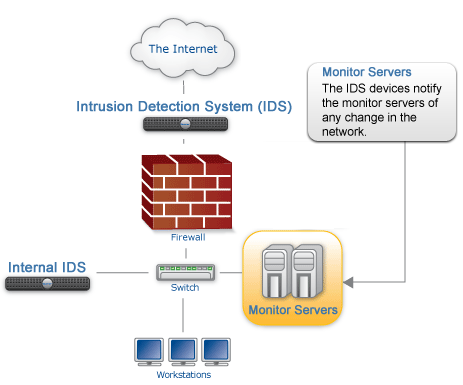
\includegraphics[width=0.6\textwidth]{Figures/idsdiagram}
\decoRule
\caption[Possible placement of IDS]{An IDS can for example be placed within the network or just before the network.}
\label{fig:IDS}
\end{figure}
\subsection{Host-based Intrusion Detection Systems}
Host-based intrusion detection systems are systems that monitor the device on which they are installed. The way they monitor the system can range from monitoring the state of the main system through log files, to monitoring program execution. In this way they can be quite indistinguishable from Anti-Virus programs.

\subsection{Network-based Intrusion Detection Systems}
Network-based intrusion detection systems are placed at certain points within a network in order to monitor traffic from and to devices within the network. The system can analyse the traffic using multiple techniques to determine whether the data is malicious. There are two different ways to analyse the network data. The analysis can be packet-based or flow-based.\\
\\
Packet-based analysis uses the entire packet including the headers and payload. An intrusion detection system that uses packet-based analysis is called a packet-based network intrusion detection system. The advantage of this type of analysis is that there is a lot of data to work with. Every single byte of the packet could be used to determine whether the packet is malicious or not. The disadvantage is immediately obvious once we look at networks through which a lot of data passes, such as data centers. Analysing every byte is very work-intensive and near impossible to do in such environments. \cite{alaidaros2011overview} \\
\\
Flow-based analysis doesn't use individual packets but uses general data about network flows. An intrusion detection system that uses flow-based analysis is called a flow-based network intrusion detection system. A flow is defined as a single connection between the host and another device. A flow can be defined using a (source\_IP, destination\_IP, source\_port, destination\_port) tuple. However flowdata also contains other information such as the duration of the connection, the start time, the amount of bytes and/or packets within the flow. Flow data can even contain data such as the amount of SYN packets within the flow. This could be useful to detect SYN overflow attacks. However not every flow collector collects this data Since flow data is much more compact than all the individual packets, it is much more feasable for data centers to use flow-based intrusion detection systems. 

\subsection{Intrusion Prevention Systems}
An intrusion prevention system or IPS/IDPS is an intrusion detection system that also has to ability to prevent attacks. An IDS does not necessarily need to be able to detect attacks at the exact moment they occur, although it is preferred. An IPS needs to be able to detect attacks real-time since it also needs to be able to prevent these attacks. For network attacks these prevention actions could be closing the connection, blocking an IP, limiting the data throughput.

\section{IP Flows}
\label{export}
Flows are aggregated from all packet data that travels through the network. Flow exporters are programs which collect network packets and aggregate them into flow records. A flow is not the same as a TCP connection. A flow can be any communication between two devices with any protocol. Flows are defined using a (source\_IP, destination\_IP, protocol) tuple. This is why flows are also called IP Flows.\\
\\
Since flow data does not contain any payload information, intrusion detection systems that use flow data cannot detect malicious behaviour embedded within payload data. \cite{IPFlow}

\section{Detection}
There are mutliple different methods to detect intrusions. There are \textbf{Signatures based methods} and there are \textbf{Anomaly Based} methods. Both of these methods have their own strengths and weaknesses. \cite{methods}
\subsection{Signature based methods}
\begin{figure}[H]
\centering
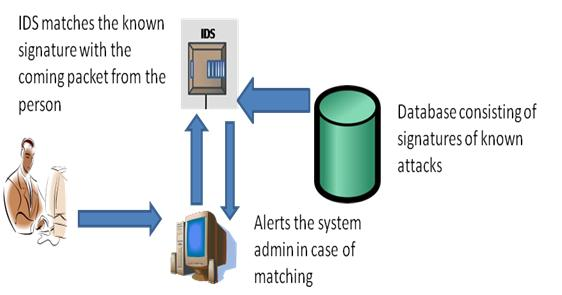
\includegraphics[width=0.7\textwidth]{Figures/Signature-based-Intrusion-Detection-System}
\decoRule
\caption[Signature based IDS]{An Signature-based intrusion detection system.}
\label{fig:Signature}
\end{figure}
\noindent Signature based methods compare so called "signatures" with an existing database of signatures. An packet or flow record is decomposed into features that together construct a signature. If the signature of an incoming flow or packet matches with a signature in the database, it is flagged as malicious. Signature-based methods have little overhead in both computation and preprocessing as it only tries to match incoming signatures to known signatures in the database. Because it only compares signatures, it is easy to deploy within a network. The system does not need to learn what the traffic within a network looks like. \\
\\
Signature based methods are very effective against known attacks. New attacks cannot be detected unless the database is updated with new signatures. It is also for attackers to avoid being caught by signature based methods, only slight modification of the "signature" is required in order to bypass the exact matching. Updating the signature database requires a lot of technical effort, since new attacks are discovered all the time.
\subsection{Anomaly based methods}
\begin{figure}[H]
\centering
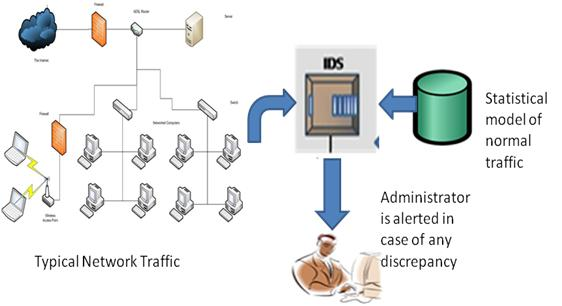
\includegraphics[width=0.7\textwidth]{Figures/Anomaly-based-Intrusion-Detection-System}
\decoRule
\caption[Anomaly based IDS]{An Anomaly-based intrusion detection system.}
\label{fig:Anomaly}
\end{figure}
\noindent Anomaly based methods, also called Behaviour based methods are methods in which the IDS tries to model the behaviour of network traffic. When an incoming packet deviates from this model, it is flagged as malicious and an alert is send. Because they use a statistical model of normal behaviour, they should be able to detect all deviations from this normal behaviour. As a result, new attacks that deviate to much from normal behaviour are detected aswell. \\
\\
Since a model of the network traffic needs to be created, the system cannot be deployed into a network and be expected to work. The system needs to learn the behaviour of the network traffic. Problems, such as generating a lot of false positive alarms, can arise when training data includes mistakes, such as misclassifications. \\
\\
Machine learning algorithms can be used as a anomaly based method. Machine learning techniques have the ability to learn from data and decide whether new data is malicous. 
% Chapter 1

\chapter{Attack Classification} % Main chapter title

\label{attack} % Change X to a consecutive number; for referencing this chapter elsewhere, use \ref{ChapterX}

An intrusion detection system can use multiple methods to detect malicious behaviour. In order to make the IDS as effective as possible, the exact classifications of attacks that can be detected need to be known.

\section{Classification}
There are several types of attacks that can occur. Some of these attacks occur from within the network, other from outside the network. The exact classifications are not mutually exclusive. Some types of malware utilise network attacks. However it is important to make a distinction between these attacks. Every attack is identified by different characteristics. Knowing these characteristics is useful to be able to tweak the IDS to make identification more effective.

\section{Network attacks}
There are \textbf{Physical attacks}, these are attacks which attempt to destroy physical equipment and hardware. \textbf{Buffer overflows} are attacks that try to execute arbritrairy code or crash a process by overflowing a buffer on the targeted system. \textbf{Password attacks} attempts to break into a system by gaining the password that the system uses. The simplest password attacks are brute-force password crackers. \textbf{DDOS} attacks are attacks which attempt to make a network resource temporarily or permanently unavailable for the users of that resource. An attack could happen by flooding a system with TCP SYN packets. \textbf{Network scans} are information gathering attacks. They do not cause any damage by themselves but usually serve the purpose to gather information about a system that could be used in further attacks. Network traffic sniffing or port scans are examples of network scans. \cite{IPFlow}

\section{Malware}
There are several types of malware. There are four distinct categories of malware. There are \textbf{botnets}, \textbf{viruses}, \textbf{trojan horses} and \textbf{worms}. Malware are actual programs that infect a system to execute a specific task. The task of the malware defines which category the malware belongs in.\\
\\
\textbf{Trojan horses} are programs disguised as harmless applications but contain malicious code. \textbf{Worms} are programs that replicate themselves among a network.  They can spread extremely fast. \textbf{Viruses} are similar to worms. However they only replicate themselves on the infected host computer. Thus they require user interaction in order to be spread around a network. The virus can accomplish this by attaching itself to an email-attachment, embed itself within an executable, etc. \\
\\
\textbf{Botnets} is malware that causes infected computers to become "slaves" to the master. An infected computer is controlled externally by the bot-master without the knowledge of the owner of the infected computer. The bot-master can use the distributed network of "slave" computer to perform other malicious tasks, such as performing an DDOS attack. \cite{IPFlow}

\section{Detection}
An NIDS only monitors the network. As such not every attack can be detected by an NIDS. Only the attacks that actually use the network can be detected. Flow-based IDS have the additional constraint that they can only use flow data. This further limits the attacks that can be detected. The attacks that can be detected using a flow-based network intrusion detection systems are:
\begin{itemize}
\item DDOS
\item Network scans
\item Worms
\item Botnets
\end{itemize}
Other attacks either do not use network communication, or they are not visible within the header information of network traffic. In order to detect other attacks, including \textbf{viruses}, \textbf{trojan horses} and \textbf{Buffer overflows}, other detection systems such as HIDS or Packet-based NIDS should be used.

\subsection{Distributed Denial of Service}
A distributed denial of service can be detected by the amount of data that is being received. However, there are many different types of DDoS attacks. There are ICMP floods, SYN floods, etc. These attacks can be described in terms of traffic patterns. A traffic pattern is expressed in a couple features. These features include the number of flows and packets, the packet size, and the total bandwidth used during the traffic. For example UDP flooding can be characterised by a traffic pattern which contains a lot of packets. These patterns can be searched for during the detection phase. \cite{kim2004flow}
\subsection{Network scans}
There are three categories of network scans.
\begin{itemize}
\item Horizontal scans: a single port is scanned across many different devices.
\item Vertical scan: several different ports are scanned on a single device
\item Block scan: a combination of both a vertical and a horizontal scan.
\end{itemize}
\noindent Scans can also be described using traffic patterns. They are characterised with a high number of flow and a low number of packets. These can again be used to detect whether a vertical or horizontal scan occurs. \cite{IPFlow} \cite{kim2004flow}

\subsection{Worms}
Worms exhibit different behaviour depending on their current state. There are two different states, a target discovery state and a transfer state. In the target discovery state, the worm explores the network to find vulnerabilities and a host to infect. During the transfer state, the worm actually transfers itself to the targeted host. The Sapphire/Slammer worm is an example of this type of behaviour. \cite{moore2003inside}\\
\\
Since transfering of the worm itself happens within the payload data, a flow-based NIDS cannot detect this state. The target discovery state can be detected. Worms use techniques similar to network scans in order to find vulnerable hosts. So similar detection techniques can be used to detect worms. \cite{abuadlla2014flow}

\subsection{Botnets}
Botnets usually consist out of a huge amount of infected slaves controlled by a central bot-master. Locating the individual infected slaves and isolating them is a difficult problem but is also insignificant due to the huge amount of remaining slaves. Detecting the bot-master and isolating that device is key to taking down a botnet. However indentifing botnet behaviour is a far more difficult problem than detection other types of malicious activities. \cite{zhu2008botnet} Malicious behaviour alone is not enough to detect botnets. \\
\\
Botnets often use IRC channels in order to communicate between slaves and the bot-master. These can be indentified using flows since they often use specific ports. It is possible to use a method that does not require specific port numbers. This requires flows including extra information such as the number of packets for which the PUSH flag is set.  


 
% Chapter 1

\chapter{Machine learning} % Main chapter title

\label{Chapter2} % Change X to a consecutive number; for referencing this chapter elsewhere, use \ref{ChapterX}

\section{What is machine learning}
Machine learning is ... .

\section{Machine learning algorithms}

\section{Supervised learning}
\subsection{Classification}
Uses discrete categories
\subsection{Regression}

\section{Unsupervised learning}
\subsection{Clustering} 
% Chapter 1

\chapter{Machine learning for an IDS} % Main chapter title

\label{Chapter3} % Change X to a consecutive number; for referencing this chapter elsewhere, use \ref{ChapterX}

\section{Using ML for an IDS}
An intrusion detection system has to detect whether some data it receives is either malicious or regular web traffic. This can be seen as a classification problem which means an machine learning algorithm for classification could be used. It needs to be determined whether data is either normal network traffic or malicious behaviour. \\
\\
Some parameters have to be chosen that will be feed into the machine learning algorithm.

\section{Disadvantages of using ML for an IDS}
\subsection{Problems}
As said before, machine learning for an intrusion detection system is a classification problem. More precisely, it can be said that intrusion detection systems have to detect abnormal behaviour in a network with mostly normal behaviour. There are several problems that can be encountered when using machine learning techniques.\\
\\
The first problem is the ability to detect new attacks. A machine learning algorithm compares incoming data with a model that it has created internally. An new type of malicious behaviour might appear to be closer to normal network traffic as compared to the model of known attacks. \\
\\
Another problem is the diversity of network traffic. The notion of "normal network traffic" is difficult to actually define. The bandwidth, duration of connections, origin of IP addresses, applications used can vary enormously through time. This makes it quite difficult for machine learning algorithms to distinguish between "normal network traffic" and malicious behaviour.\cite{ClosedWorld} 

\subsection{Solutions}
There are several solutions that can be used in order to make machine learning algorithms more effective for intrusion detection systems. One option is to chance the way the classification problem is defined. Instead of defining the classes, "normal" and "malicious", there might be different classes for different types of malicious behaviour. In the same way, different classes can be defined for different types normal traffic. 

%\include{Chapters/Chapter5} 

%----------------------------------------------------------------------------------------
%	THESIS CONTENT - APPENDICES
%----------------------------------------------------------------------------------------

\appendix % Cue to tell LaTeX that the following "chapters" are Appendices

% Include the appendices of the thesis as separate files from the Appendices folder
% Uncomment the lines as you write the Appendices

% Appendix A

\chapter{Appendix Title Here} % Main appendix title

\label{AppendixA} % For referencing this appendix elsewhere, use \ref{AppendixA}

Write your Appendix content here.
%\include{Appendices/AppendixB}
%\include{Appendices/AppendixC}

%----------------------------------------------------------------------------------------
%	BIBLIOGRAPHY
%----------------------------------------------------------------------------------------

\printbibliography[heading=bibintoc]

%----------------------------------------------------------------------------------------

\end{document}  
